\section{Pre-study}
\thispagestyle{plain}
	\subsection{Solution today}
		\subsubsection{Existing functionality}
Since the application already is considered a working prototype, we will provide a list which gives a description for the functionality. Working functionality is in this report defined as the functionality that is implemented in the front-end or back-end. If something is implemented back-end it has to be used front-end. A more detailed technical description is found in the architecture-section.

\begin{figure}[h!]
\begin{center}
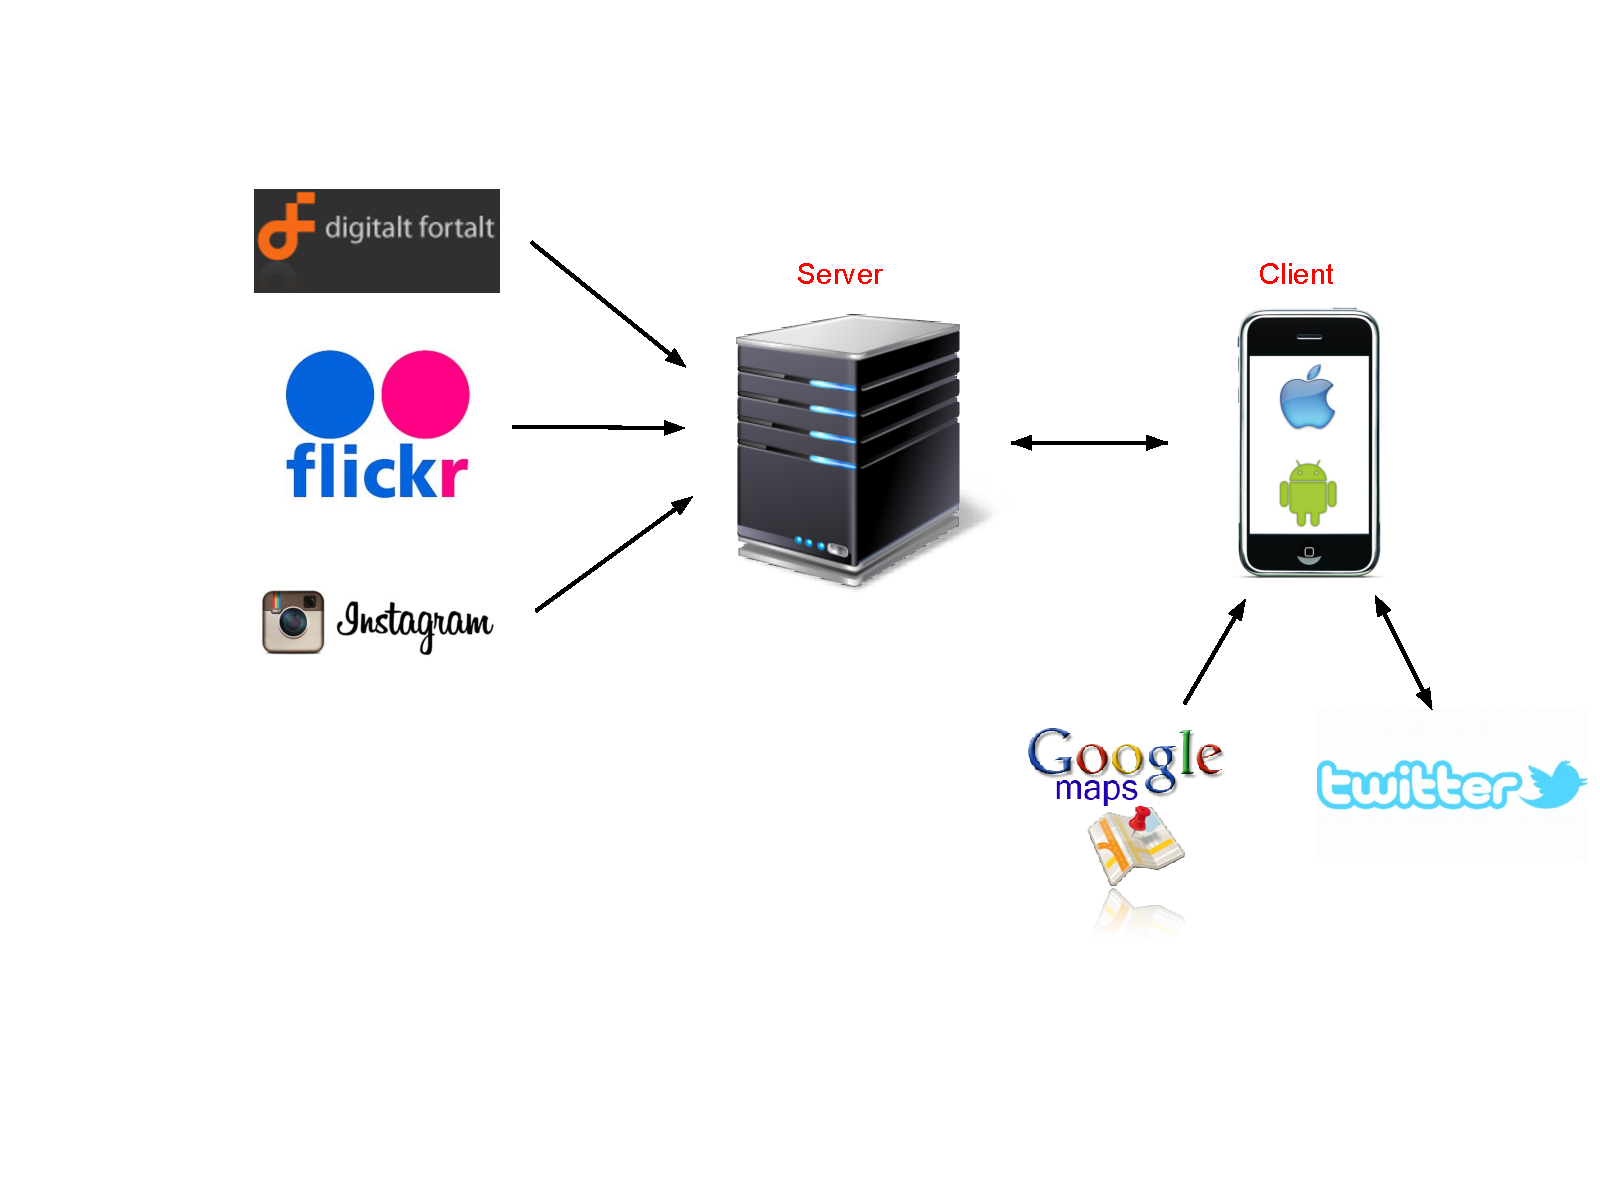
\includegraphics[scale=0.45]{ntoverview-architecture}
\caption{A simple overview of the architecture}
\end{center}
\end{figure}

\begin{itemize}
\item Browse a map and zoom in and out.
\item Load \textbf{places}.
\item Click on a place in the map and access \textbf{stories} from Digitalt Fortalt.
\item Get social media related to a place from the content providers Instagram and Twitter.
\item Go to a users exact position on a map.
\item Search for a location in the map.
\end{itemize}
	
		\subsubsection{Limitations}
There are some limitations to the system that needs to be further developed, and some that probably would require total architectural review of the project to be fixed. Our task is to continue the development of the application. An overview of the features we are going to improve are discussed in the requirements section \ref{sec:Reqs}. 

		\subsubsection{App evaluation}
		
After the first meetings we concluded that the best way to proceed is to evaluate the existing system, to uncover potential issues and flaws.
Therefore we decided that everyone should individually do a usability test when exploring the app for the first time. Here is a short summary of all our reports:

The first major issue most of us experienced is how slow the app loads, with no feedback that something is actually working in the background. Another thought that generally comes to mind is \emph{I don't understand the apps function when opening it without prior knowledge}. What happens is that you get a map with tags you could click on, making you believe the function of the app is to use it when visiting a town (not Trondheim in particular) and want to explore historical monuments and get Wikipedia facts. When clicking on tags you get to the location-specific page, with content from Instagram. Some of us found this social feature not to have very obvious intentions. The social integration seemed out of place. You would want actual and useful information about places to be displayed first. One could also get confused when suddenly a lot of Instagram photos with random people suddenly appear. Our first impression is that this social aspect have to offer something more interesting to be relevant at this stage. 
\\
There is a nice touch with a slight gradient in the bottom indicating that you can scroll down for more content. When the phone is turned (switched to landscape mode) there are issues however. There is no scroll function here limiting the content available and the images are cropped. Also, if there is a lot of text added in the Instagram feed, it disappears along with the hashtags. The way to collect images from Instagram to the application also seems to be sub optimal when irrelevant content are displayed. When tweeting there are no limitations on length, which causes problems when trying to post tweets over 140 characters.\\
\\
These are some of the feedback extracted from the individual tests. 

		
	\subsection{Survey}


	One of the most important research we did during the pre-study was to conduct interviews about Stedr. In these interviews we let six everyday people, use the current version of Stedr and paid close attention to how they used it. The subjects was both male and female raging between 18-30 in age. The main purpose of this interview session was to get feedback on proposed features from our customer.\\*[8pt]
	Firstly, after the test subject had some time to play with the app. We asked asked some questions about social media integrations, and this is the results:\\

	\emph{Can you see yourself tweeting about a place from Stedr?}\\
	Yes: \textbf{0}\hspace{0.5cm}
	No: \textbf{3}\hspace{0.5cm}
	Don't know: \textbf{3}\\[6pt]
	
	\emph{What about Instagram?}\\
	Yes: \textbf{0}\hspace{0.5cm}
	No: \textbf{3}\hspace{0.5cm}
	Don't know: \textbf{3}\\[6pt]
	
	\emph{What about SoundCloud?}\\
	Yes: \textbf{0}\hspace{0.5cm}
	No: \textbf{4}\hspace{0.5cm}
	Don't know: \textbf{2}\hspace{0.5cm}\\[6pt]

	Additionally, we asked about Wikipedia. This was a proposition from us.\\*[8pt]
	\emph{Would you like the app better if Wikipedia was integrated?}\\
	Yes: \textbf{6}\hspace{0.5cm}
	No: \textbf{0}\hspace{0.5cm}
	Don't know:  \textbf{0}\\*[8pt]
	In retrospect, we see that even though people were positive to this, it doesn't really fit into what Stedr is about. Because of this, we abounded this feature late on.\\
	
	When asked if they can envision using the app in the future, this was their responses:
\begin{itemize}
	\item ”Yes, if the app can also show patios.”
	\item ”Unfortunately, I don't use social media that much, but if the app was more historically oriented, I would be intrigued to use it.”
	\item ”Yes totally!”
	\item ”It must be better than Google Maps for me to bother using it. I want the social features, but only for contributing, not for looking at what other people write. I would also use twitter with the app, but only if there was pre defined tweets.”
	\item”Maybe, if I knew about it.”
	\item ”Yes, it sounds like a good idea.”
\end{itemize}

	The general consensus was very positive about Stedr. Everyone liked the idea, but some were sceptical in regards to the social features that was purposed.

	In response to these results, our customer thought this survey was interesting, but it did not change her mind about trying out these features, in part because she had previously organized focus groups with other results. We respect this decision of course, but feel that it was right of us to do this reaserach regardless.
	
	\subsection{Tools and technologies}
	
		\subsubsection{APIs}
		

		There was a wish from the customer that we should use other existing services as mush as possible instead of having our own database and a comprehensive back-end. The result of this is that the project will be dependent on many different APIs to function properly. As a result of this we spent a lot of time researching different APIs. The existing system had already Norvegiana, Flickr, Instagram and Twitter, though some of them needed a fresh up. In addition, our customer had ideas to expand functionality which meant more APIs. We did research on a lot of different APIs like Google Places, Wikipedia, NRK but did not end up using any of them after consulting with our customer. 
		
\paragraph{Digitalt Fortalt and Norvegiana.}

After a evaluation in the pre-study phase we decided to switch the main API of application for better performance. Here is a short summary of why:

In current condition, Stedr uses an API called Norvegiana. This API is basically a collection of all public APIs that can be used in collecting different data. The major pros using Norvegiana is the portion of information accessible from different sources including \emph{Statsarkivet, Digitalt Fortalt, Digitalt Museum} etc. There are many filtering options making Norvegiana able to return all the information needed.

There has been some complaints about how the current service works. Norvegiana is an interface to the dissemination system, not the production system. Which means that when a story is created, one has to wait for the Art Council Norway to perform an export from production to dissemination. This means that stories are not available through Norvegiana at once after they are produced. In some case we had to wait a few weeks. This is not acceptable with respect to our goal of increasing user participation and enhancing usability. We think this problem might be solved by switching completely to the Digitalt Fortalt API, which should not be too much trouble considering the existing code only makes simple calls to the API trough Norvegiana. It is worth noting that Digitalt Fortalt is originally meant for Norwegian cultural heritage, which might cause problems in a potential international expansion.

The functionality in the APIs, for our usage, are about the same. Where both come short is that both strictly speaking work like databases that you only can retrieve information from, making them impossible to use for posting new content. This has to be solved in another way.

	\subsection{Similar products}
		
As a part of this project we have reviewed apps that come close to our own in regards to purpose, target groups and functionality. One of the apps we looked at is Trondheim Guide.

One of the best features of Trondheim Guide is virtual reality, where you can look into the screen and see what you have in front of you. This can for instance be used to see the distance to the nearest cultural heritage or attractions. You can also have your own journal, where you can add places you have been to. This is tracked with time and date. There is also an very nice feature where you can make your own postcard, and share it with friends. For each place you visit you can check in with both comments and picture, this is saved in your log as well. Although Trondheim Guide is first and foremost an tourist app, it can also be used to discover various cultural heritages around Trondheim.

Another app that overlaps a lot with ours is KNappen. KNappen is an aesthetically pleasing, well-designed app with a user-friendly GUI. Like our own app it is focused around places. You will find images, routes, augmented reality, audio, video and informative and historical texts related to places. Users can also see the Wikipedia article about the place and they can see related places. They have a map view that is somewhat similar the one in our app, where icons are used to represent the different places.


\begin{figure}[h!]
\begin{center}
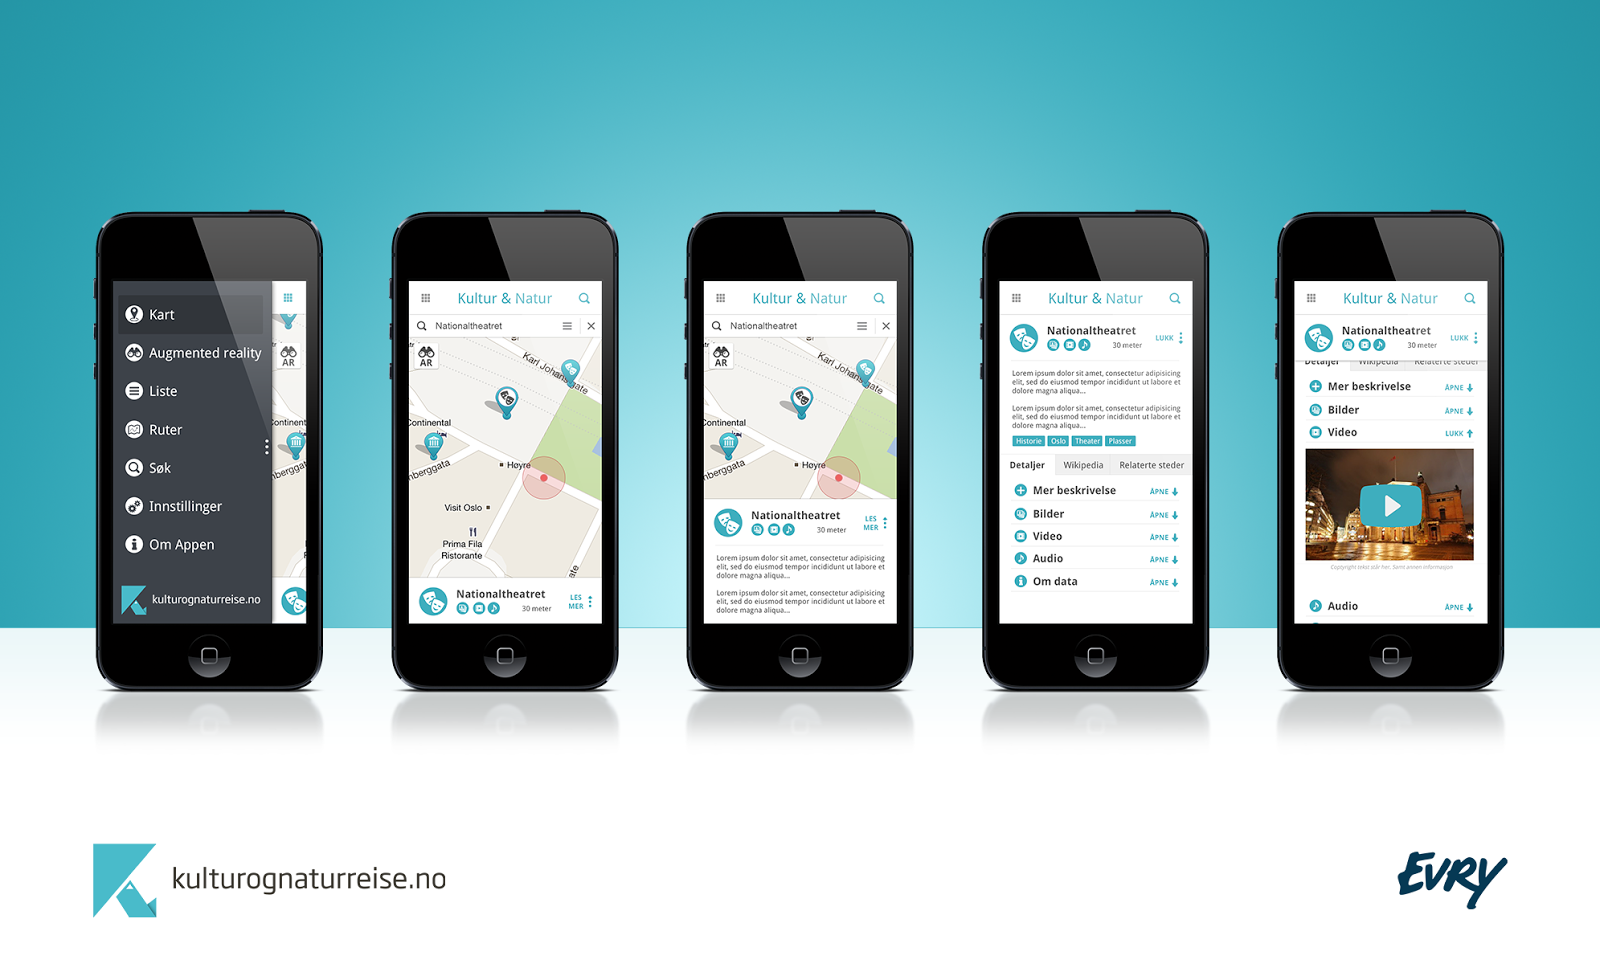
\includegraphics[width=1\textwidth]{res/image02.png}
\caption{KNappen screenshots}
\end{center}
\end{figure}


We think Stedr could benefit from implementing some of the features from these two apps. Especially virtual reality from Trondheim Guide would be a great addition to the app. The user experience from KNappen is also something Stedr could take some inspiration from
